\documentclass[12pt,a4paper]{article}
\usepackage[utf8]{inputenc}
\usepackage{amsmath}
\usepackage{amsfonts}
\usepackage{amssymb}
\usepackage[brazil]{babel}
\usepackage{indentfirst}
\usepackage{url}
\usepackage{float}
\usepackage{color}
\usepackage{colortbl}

\definecolor{pblue}{rgb}{0.13,0.13,1}
\definecolor{pgreen}{rgb}{0,0.5,0}
\definecolor{pred}{rgb}{0.9,0,0}
\definecolor{pgrey}{rgb}{0.46,0.45,0.48}
\definecolor{cinzaClaro}{rgb}{0.9,0.9,0.9}

\definecolor{mygreen}{rgb}{0,0.6,0}
\definecolor{mygray}{rgb}{0.5,0.5,0.5}
\definecolor{mymauve}{rgb}{0.58,0,0.82}

\RequirePackage{graphicx}
\title{Dicionário de Dados}
\author{Gusttavo Nunes Gomes\and Jonathan Silvestre Sousa \and Salmi Nunes de Paula Junior\and Willian Wallace de Matteus Silva}
 
\usepackage[left=3cm,right=3cm,top=2cm,bottom=2cm]{geometry}
\begin{document}
\begin{titlepage}
\begin{center}
\begin{figure}[htb]
                
                \label{figura:LogoIF}
        
                \centering
                \includegraphics[width=6cm]{recursos/imagens/logo.png} 
\end{figure}
Instituto Federal Goiano - Campus Ceres\\
Bacharelado em Sistemas de Informação\\
Prof. Me. Ronneesley Moura Teles\\\vspace{1cm}

Gusttavo Nunes Gomes\\
Jonathan Silvestre Sousa \\
Salmi Nunes de Paula Junior\\
Willian Wallace de Matteus Silva\\
\vspace{6.0cm}
\textit{\textbf{\Large{Dicionário de Dados}}}\\\vspace{11cm}
Novembro\\
2017\\
\end{center}
\end{titlepage}
\tableofcontents
\newpage
\begin{center}
\textbf{\Large{Dicionário de Dados}}\\\vspace{0.5cm}
\end{center}
\section{Dicionário de Dados (DD)}


No processo de análise de sistemas um dos pontos fortes é o MER (modelo de entidade de relacionamento). Onde e definidas as relações entre as entidades.

Juntamente com o modelo de entidade de relacionamento, é necessario que se tenha uma documentação com a explicação de todo os campos do banco de dados. Este documento e chamado de dicionário de dados (DD), onde contem informações textuais sobre os dados permitindo um maior entendimento de todos os campos.

O dicionário de dados e composto de uma lista organizada contendo todos os elementos de dados que são pertinentes para o sistema. Sem o dicionário de dados o modelo não pode ser considerado completo, pois este descreve entradas, saídas, composição de depósitos de dados e alguns cálculos intermédios. O DD consiste num ponto de referência de todos os elementos envolvidos na medida em que permite associar um significado a cada termo utilizado.


\subsection{Dados elementares}
Os dados elementares correspondem a elementos atómicos, ou seja, elementos sem decomposição no contexto do utilizador.
Exemplo: Apesar de se utilizar o N\_telefone, como um exemplo de descrição de um elemento de dados composto, na maior parte dos contextos este dado é considerado elementar.

O DD permite inventariar e descrever os seguintes itens:
\begin{itemize}
	\item Depósitos de dados;
	\item Fluxos de dados;
	\item Dados elementares que constituem fluxos e depósitos de dados;
\end{itemize}
Cada entrada no DD é constituída por um identificador e respectiva descrição. A descrição de cada entrada inclui:


\begin{itemize}
	\item O seu significado;
	\item O seu conteúdo (só para dados compostos);
	\item Os valores permitidos e unidades (só para dados elementares);
	\item A chave primária (só para depósitos de dados).
\end{itemize}

\subsection{Notação utilizada no DD}

Para descrever de uma forma precisa cada componente de dados e utilizado um conjunto de símbolos simples.

\begin{center}
\begin{table}[h!]
	
	\label{tabela:tiposAtividades}
	%%%%%%%%%%%%%%%%%%%%Estrutura Tabela%%%%%%%%%%%%%%
	\begin{tabular}{|p{2.5cm}|p{13.5cm}|}\hline	
		\multicolumn{2}{|p{17cm}|}{\cellcolor{cinzaClaro}  \centering Notação utilizada no DD} \\ \hline %Parte superior da Tabela
		 \textbf{Símbolo}   &  \textbf{Significado} \\\hline %Parte com os nomes de cada Coluna
	%%%%%%%%%%%%%%%%%%%%Estrutura Tabela%%%%%%%%%%%%%%
		
		 =  & é constituído por ou é definido por \\\hline
		  +   &  e (conjunção ou concatenação)\\\hline
		   ( )   &  enquadram componentes opcionais\\\hline
		    [ ]  & enquadram componentes que são utilizadas alternativamente \\\hline
		     $\vert$  & separam componentes alternativas enquadradas por [ ] \\\hline
		      $\lbrace  \rbrace$  & enquadram componentes que se repetem 0 ou mais vezes \\\hline
		       **  & enquadram comentários\\\hline
		        @  & identifica a chave primária de um depósito \\\hline
			
	\end{tabular}
	\caption{Notações utilizadas no DD}
\end{table}	
\end{center}

Exemplos:

\begin{itemize}
\item Descrição de um elemento de dados composto:
\end{itemize}

N\_telefone = (indicativo\_internacional + indicativo\_país)	+ ( indicativo\_zona ) + $N^{o}$\_assinante

indicativo\_internacional =$\lbrace$dígito$\rbrace$

indicativo\_país =$\lbrace$dígito$\rbrace$

indicativo\_zona =$\lbrace$dígito$\rbrace$

$N^{o}$\_assinante =$\lbrace$dígito$\rbrace$\\\\



Dígito = [ 0 $\vert$ 1 $\vert$ 2 $\vert$ 3 $\vert$ 4 $\vert$ 5 $\vert$ 6 $\vert$ 7 $\vert$ 8 $\vert$ 9 ]


\begin{itemize}
\item Descrição de elementos de dados elementares: Sexo = * Valores: [ M $\vert$ F ] *
Peso = \\ * Peso do paciente quando é admitido no hospital *\\
* Unidades: Kg Intervalo: 1-150*
\end{itemize}

\subsection{Exemplos de Dicionários de Dados}

O exemplo apresentado corresponde a uma parte do DD do sistema de Gestão  de Bibliotecas e inclui a descrição dos seguintes itens:

\begin{itemize}
\item O fluxo de dados Ficha\_leitor;
\item O depósito de dados Leitor;
\item Alguns dos dados elementares dos itens anteriores.
\end{itemize}
\ldots\\
BI =  *Número do Bilhete de identidade do leitor*\\
Data\_admissão = *Data de inscrição do leitor*\\\\

Ficha\_leitor = *Dados pessoais do leitor fornecidos para a sua inscrição ou alteração de informação*\\


(N\_leitor) + Nome + Morada + BI + Telefone + Profissão\\

Leitor = $\lbrace$Leitor\_i$\rbrace$\\

Leitor\_i = *Informação mantida sobre cada leitor da biblioteca*

@N\_leitor + Nome + Morada + BI + Telefone + Profissão + Data\_admissão\\

N\_leitor = *Número de identificação de leitor da Biblioteca* 		$\lbrace$dígito$\rbrace$\\

O exemplo mostrado abaixo e o metodo escolhido para ser utilizado na construção do dicionario de dados da rede social onde comtem entidade, campo físico, chave, tipo, tamanho, nulo e descrição.


\begin{center}
\begin{table}[h!]
	\label{tabela:exemplo}
	%%%%%%%%%%%%%%%%%%%%Estrutura Tabela%%%%%%%%%%%%%%
	\begin{tabular}{|p{2.3cm}|p{1.2cm}|p{1.8cm}|p{1.5cm}|p{1cm}|p{6cm}|}\hline	
		\multicolumn{6}{|p{16cm}|}{\cellcolor{cinzaClaro}  \centering Tabela: \texttt{usuarios}} \\ \hline %Parte superior da Tabela
		{\small Campo Físico}   & {\small Chaves} & {\small Tipo} & {\small Tamanho} & {\small Nulo} & {\small Descrição}\\\hline %Parte com os nomes de cada Coluna
	%%%%%%%%%%%%%%%%%%%%Estrutura Tabela%%%%%%%%%%%%%%
		
		{\tiny id} & {\tiny PK} & {\tiny INT} & {\tiny } & {\tiny Not Null} &{\tiny Id do usuário}\\\hline
		{\tiny nome} & {\tiny } & {\tiny VARCHAR} & {\tiny 200} & {\tiny Not Null} &{\tiny  Nome do usuário}\\\hline
		{\tiny email} & {\tiny } & {\tiny VARCHAR} & {\tiny 200} & {\tiny Not Null} &{\tiny Email do usuário}\\\hline
		{\tiny telefone} & {\tiny } & {\tiny VARCHAR } & {\tiny 18} & {\tiny  Null} &{\tiny Telefone do usuário}\\\hline
		{\tiny senha} & {\tiny } & {\tiny CHAR} & {\tiny 32} & {\tiny Not Null} &{\tiny Senha do usuário}\\\hline
		{\tiny data\_nascimento} & {\tiny } & {\tiny DATE} & {\tiny } & {\tiny Not Null} &{\tiny Data de nascimento do usuário}\\\hline
		{\tiny sexo} & {\tiny } & {\tiny CHAR} & {\tiny 1} & {\tiny Not Null} &{\tiny Sexo do usuário}\\\hline
		{\tiny data\_cadastro} & {\tiny } & {\tiny DATETIME} & {\tiny } & {\tiny Not Null} &{\tiny Data e hora de cadastro do usuário}\\\hline
		{\tiny status} & {\tiny } & {\tiny BOOL} & {\tiny } & {\tiny Not Null} &{\tiny Status do usuário, se está ativo ou inativo}\\\hline		
		{\tiny foto} & {\tiny FK} & {\tiny INT} & {\tiny } & {\tiny Not Null} &{\tiny Foto vinculada ao perfil do usuário}\\\hline
		{\tiny cidade} & {\tiny FK} & {\tiny INT} & {\tiny } & {\tiny Not Null} &{\tiny Id da cidade do usuário}\\\hline
		
			
	\end{tabular}
\end{table}	
\end{center}

Analisando a tabela acima teremos:

\begin{itemize}
\item \textbf{Entidade}: é o nome da entidade que foi definida no MER. A entidade é uma pessoa, objeto ou lugar que será considerada como objeto pelo qual temos interesse em guardar informações a seu respeito.

\item \textbf{Campo Físico}: é utilizado para o armazenado do nome dos campos.

\item \textbf{Chave}: campo utilizado para o armazenamento do tipo de chave.

\item \textbf{Tipo}: descreve o tipo do campo podendo ser ele numérico, textual, data ou boleano.

\item \textbf{Nulo}: utilizado para descrever se o campo pode ou não ser nulo.

\item \textbf{Tamanho}: define a quantidade de caracteres que podem ser marzenados neste campo.

\item \textbf{Descrição}: é opcional e pode ser usado para descrever o que é aquele campo armazena.
\end{itemize}

\newpage
\section{Dicionário de Dados - Rede Social}
\subsection{Eventos}

\begin{center}
\begin{table}[h!]
	\caption{\texttt{tipos\_atividades}}
	\label{tabela:tiposAtividades}
	%%%%%%%%%%%%%%%%%%%%Estrutura Tabela%%%%%%%%%%%%%%
	\begin{tabular}{|p{2.3cm}|p{1.2cm}|p{1.8cm}|p{1.5cm}|p{1cm}|p{6cm}|}\hline	
		\multicolumn{6}{|p{16cm}|}{\cellcolor{cinzaClaro}  \centering Tabela: \texttt{tipos\_atividades}} \\ \hline %Parte superior da Tabela
		{\small Campo Físico}   & {\small Chaves} & {\small Tipo} & {\small Tamanho} & {\small Nulo} & {\small Descrição}\\\hline %Parte com os nomes de cada Coluna
	%%%%%%%%%%%%%%%%%%%%Estrutura Tabela%%%%%%%%%%%%%%
		
		{\tiny id}   & {\tiny PK} & {\tiny INT} & {\tiny } & {\tiny Not Null} &{\tiny Código do tipo de atividade.}\\\hline
		{\tiny nome}  & {\tiny } & {\tiny VARCHAR} & {\tiny 100} & {\tiny Not Null} &{\tiny Nome do tipo de atividade}\\\hline
		{\tiny restricao} & {\tiny } & {\tiny BOOLEAN} & {\tiny } & {\tiny Not Null} &{\tiny Restrição sobre determinada tipo de atividade (Aberta ou Fechada)}\\\hline
		
		%{\tiny } & {\tiny } & {\tiny } & {\tiny } & {\tiny } &{\tiny }\\\hline %Modelo de novas linhas
			
	\end{tabular}
\end{table}	
\end{center}


\begin{center}
\begin{table}[h!]
	\caption{\texttt{atividades}}
	\label{tabela:atividades}
	%%%%%%%%%%%%%%%%%%%%Estrutura Tabela%%%%%%%%%%%%%%
	\begin{tabular}{|p{2.3cm}|p{1.2cm}|p{1.8cm}|p{1.5cm}|p{1cm}|p{6cm}|}\hline		
		\multicolumn{6}{|p{16cm}|}{\cellcolor{cinzaClaro}  \centering Tabela: \texttt{atividades}} \\ \hline %Parte superior da Tabela
		{\small Campo Físico}   & {\small Chaves} & {\small Tipo} & {\small Tamanho} & {\small Nulo} & {\small Descrição}\\\hline %Parte com os nomes de cada Coluna
	%%%%%%%%%%%%%%%%%%%%Estrutura Tabela%%%%%%%%%%%%%%
		
		{\tiny id}  & {\tiny PK} & {\tiny INT} & {\tiny } & {\tiny Not Null} &{\tiny Código da atividade.}\\\hline
		{\tiny nome}  & {\tiny } & {\tiny VARCHAR} & {\tiny 100} & {\tiny Not Null} &{\tiny Nome da atividade.}\\\hline
		{\tiny descricao}  & {\tiny } & {\tiny TEXT} & {\tiny } & {\tiny Not Null} &{\tiny Descrição da atividade.}\\\hline
		{\tiny inicio}  & {\tiny } & {\tiny DATETIME} & {\tiny } & {\tiny Not Null} &{\tiny Data e hora de quando começará a atividade.}\\\hline
		{\tiny vagas}  & {\tiny } & {\tiny INT} & {\tiny } & {\tiny Null} &{\tiny Quantidade de vagas para essa atividade.}\\\hline
		{\tiny evento}  & {\tiny FK} & {\tiny INT} & {\tiny } & {\tiny Not Null} &{\tiny Código do evento vinculado.}\\\hline
		{\tiny tipo}  & {\tiny FK} & {\tiny INT} & {\tiny } & {\tiny Not Null} &{\tiny Código do tipo de atividade vinculado.}\\\hline
		
			
	\end{tabular}
\end{table}	
\end{center}


\begin{center}
\begin{table}[h!]
	\caption{\texttt{presenca\_atividades}}
	\label{tabela:presencaAtividades}
	%%%%%%%%%%%%%%%%%%%%Estrutura Tabela%%%%%%%%%%%%%%
	\begin{tabular}{|p{2.3cm}|p{1.2cm}|p{1.8cm}|p{1.5cm}|p{1cm}|p{6cm}|}\hline	
		\multicolumn{6}{|p{16cm}|}{\cellcolor{cinzaClaro}  \centering Tabela: \texttt{presenca\_atividades}} \\ \hline %Parte superior da Tabela
		{\small Campo Físico}   & {\small Chaves} & {\small Tipo} & {\small Tamanho} & {\small Nulo} & {\small Descrição}\\\hline %Parte com os nomes de cada Coluna
	%%%%%%%%%%%%%%%%%%%%Estrutura Tabela%%%%%%%%%%%%%%
		
		{\tiny presenca} & {\tiny } & {\tiny BOOLEAN} & {\tiny } & {\tiny Not Null} &{\tiny Se o usuário esteve ou não presente no evento.}\\\hline
		{\tiny atividade}  & {\tiny FK} & {\tiny INT} & {\tiny } & {\tiny Not Null} &{\tiny Evento vinculado ao usuário.}\\\hline
		{\tiny usuario}  & {\tiny FK} & {\tiny INT} & {\tiny } & {\tiny Not Null} &{\tiny Usuário vinculado à atividade.}\\\hline
			
	\end{tabular}
\end{table}	
\end{center}


\begin{center}
\begin{table}[h!]
	\caption{\texttt{responsaveis\_atividades}}
	\label{tabela:responsaveisAtividades}
	%%%%%%%%%%%%%%%%%%%%Estrutura Tabela%%%%%%%%%%%%%%
	\begin{tabular}{|p{2.3cm}|p{1.2cm}|p{1.8cm}|p{1.5cm}|p{1cm}|p{6cm}|}\hline	
		\multicolumn{6}{|p{16cm}|}{\cellcolor{cinzaClaro}  \centering Tabela: \texttt{responsaveis\_atividades}} \\ \hline %Parte superior da Tabela
		{\small Campo Físico}   & {\small Chaves} & {\small Tipo} & {\small Tamanho} & {\small Nulo} & {\small Descrição}\\\hline %Parte com os nomes de cada Coluna
	%%%%%%%%%%%%%%%%%%%%Estrutura Tabela%%%%%%%%%%%%%%
		
		{\tiny atividade}  & {\tiny FK} & {\tiny INT} & {\tiny } & {\tiny Not Null} &{\tiny Atividade vinculada ao usuario responsável.}\\\hline
		{\tiny usuario} & {\tiny FK} & {\tiny INT} & {\tiny } & {\tiny Not Null} &{\tiny Usuário vinculado a atividade.}\\\hline
			
	\end{tabular}
\end{table}	
\end{center}


\begin{center}
\begin{table}[h!]
	\caption{\texttt{organizadores\_eventos}}
	\label{tabela:organizadoresEventos}
	%%%%%%%%%%%%%%%%%%%%Estrutura Tabela%%%%%%%%%%%%%%
	\begin{tabular}{|p{2.3cm}|p{1.2cm}|p{1.8cm}|p{1.5cm}|p{1cm}|p{6cm}|}\hline	
		\multicolumn{6}{|p{16cm}|}{\cellcolor{cinzaClaro}  \centering Tabela: \texttt{organizadores\_eventos}} \\ \hline %Parte superior da Tabela
		{\small Campo Físico}   & {\small Chaves} & {\small Tipo} & {\small Tamanho} & {\small Nulo} & {\small Descrição}\\\hline %Parte com os nomes de cada Coluna
	%%%%%%%%%%%%%%%%%%%%Estrutura Tabela%%%%%%%%%%%%%%
		
		{\tiny evento} & {\tiny FK} & {\tiny INT} & {\tiny } & {\tiny Not Null} &{\tiny Evento vinculado ao usuário.}\\\hline
		{\tiny usuario} & {\tiny FK} & {\tiny INT} & {\tiny } & {\tiny Not Null} &{\tiny Usuário vinculado ao evento.}\\\hline
			
	\end{tabular}
\end{table}	
\end{center}


\begin{center}
\begin{table}[h!]
	\caption{\texttt{presenca\_evento}}
	\label{tabela:presencaEvento}
	%%%%%%%%%%%%%%%%%%%%Estrutura Tabela%%%%%%%%%%%%%%
	\begin{tabular}{|p{2.3cm}|p{1.2cm}|p{1.8cm}|p{1.5cm}|p{1cm}|p{6cm}|}\hline		
		\multicolumn{6}{|p{16cm}|}{\cellcolor{cinzaClaro}  \centering Tabela: \texttt{presenca\_evento}} \\ \hline %Parte superior da Tabela
		{\small Campo Físico}   & {\small Chaves} & {\small Tipo} & {\small Tamanho} & {\small Nulo} & {\small Descrição}\\\hline %Parte com os nomes de cada Coluna
	%%%%%%%%%%%%%%%%%%%%Estrutura Tabela%%%%%%%%%%%%%%
		
		{\tiny presencao}  & {\tiny } & {\tiny BOOLEAN } & {\tiny } & {\tiny Not Null} &{\tiny Se o usuário esteve ou não presente no evento.}\\\hline
		{\tiny evento}  & {\tiny FK} & {\tiny INT} & {\tiny } & {\tiny Not Null } &{\tiny Evento vinculado ao usuário.}\\\hline
		{\tiny usuario}  & {\tiny FK} & {\tiny INT} & {\tiny } & {\tiny Not Null} &{\tiny Usuário vinculado ao evento.}\\\hline
			
	\end{tabular}
\end{table}	
\end{center}


\begin{center}
\begin{table}[h!]
	\caption{\texttt{eventos}}
	\label{tabela:eventos}
	%%%%%%%%%%%%%%%%%%%%Estrutura Tabela%%%%%%%%%%%%%%
	\begin{tabular}{|p{2.3cm}|p{1.2cm}|p{1.8cm}|p{1.5cm}|p{1cm}|p{6cm}|}\hline		
		\multicolumn{6}{|p{16cm}|}{\cellcolor{cinzaClaro}  \centering Tabela: \texttt{eventos}} \\ \hline %Parte superior da Tabela
		{\small Campo Físico}   & {\small Chaves} & {\small Tipo} & {\small Tamanho} & {\small Nulo} & {\small Descrição}\\\hline %Parte com os nomes de cada Coluna
	%%%%%%%%%%%%%%%%%%%%Estrutura Tabela%%%%%%%%%%%%%%
		
		{\tiny id} & {\tiny PK} & {\tiny INT} & {\tiny } & {\tiny Not Null} &{\tiny Id do evento.}\\\hline
		{\tiny nome} & {\tiny } & {\tiny VARCHAR} & {\tiny 100} & {\tiny Not Null} &{\tiny Nome do tipo do evento.}\\\hline
		{\tiny descricao} & {\tiny } & {\tiny TEXT} & {\tiny } & {\tiny Not Null} &{\tiny Descreve mais detalhadamente o evento.}\\\hline
		{\tiny certificado} & {\tiny } & {\tiny BOOLEAN} & {\tiny } & {\tiny Not Null} &{\tiny Diz se o evento fornece certificado.}\\\hline
		{\tiny inicio} & {\tiny } & {\tiny DATETIME} & {\tiny } & {\tiny Not Null} &{\tiny Data e hora que o evento começa.}\\\hline
		{\tiny fim} & {\tiny } & {\tiny DATETIME} & {\tiny } & {\tiny Not Null} &{\tiny Data e hora que o evento termina.}\\\hline
		{\tiny responsavel} & {\tiny } & {\tiny INT} & {\tiny } & {\tiny Not Null} &{\tiny Id do usuário que cadastrou o evento, vinculado automaticamente pelo login.}\\\hline
		{\tiny inicio\_inscricao} & {\tiny } & {\tiny DATETIME} & {\tiny } & {\tiny Not Null} &{\tiny Data e hora que abrem as inscrições para o evento.}\\\hline
		{\tiny encerramento\_inscricao} & {\tiny } & {\tiny DATETIME} & {\tiny } & {\tiny Not Null} &{\tiny Data e hora que fecham as inscrições para o evento.}\\\hline
		
		%{\tiny } & {\tiny } & {\tiny } & {\tiny } & {\tiny } & {\tiny } &{\tiny }\\\hline %Modelo de novas linhas
			
	\end{tabular}
\end{table}	
\end{center}

\subsection{Artefatos do usuários}

%Inserir as tabelas de Artefatos do usuários

\begin{center}
\begin{table}[h!]
	\caption{\texttt{usuarios}}
	\label{tabela:usuarios}
	%%%%%%%%%%%%%%%%%%%%Estrutura Tabela%%%%%%%%%%%%%%
	\begin{tabular}{|p{2.3cm}|p{1.2cm}|p{1.8cm}|p{1.5cm}|p{1cm}|p{6cm}|}\hline	
		\multicolumn{6}{|p{16cm}|}{\cellcolor{cinzaClaro}  \centering Tabela: \texttt{usuarios}} \\ \hline %Parte superior da Tabela
		{\small Campo Físico}   & {\small Chaves} & {\small Tipo} & {\small Tamanho} & {\small Nulo} & {\small Descrição}\\\hline %Parte com os nomes de cada Coluna
	%%%%%%%%%%%%%%%%%%%%Estrutura Tabela%%%%%%%%%%%%%%
		
		{\tiny id} & {\tiny PK} & {\tiny INT} & {\tiny } & {\tiny Not Null} &{\tiny Id do usuário}\\\hline
		{\tiny nome} & {\tiny } & {\tiny VARCHAR} & {\tiny 200} & {\tiny Not Null} &{\tiny  Nome do usuário}\\\hline
		{\tiny email} & {\tiny } & {\tiny VARCHAR} & {\tiny 200} & {\tiny Not Null} &{\tiny Email do usuário}\\\hline
		{\tiny telefone} & {\tiny } & {\tiny VARCHAR } & {\tiny 18} & {\tiny  Null} &{\tiny Telefone do usuário}\\\hline
		{\tiny senha} & {\tiny } & {\tiny CHAR} & {\tiny 32} & {\tiny Not Null} &{\tiny Senha do usuário}\\\hline
		{\tiny data\_nascimento} & {\tiny } & {\tiny DATE} & {\tiny } & {\tiny Not Null} &{\tiny Data de nascimento do usuário}\\\hline
		{\tiny sexo} & {\tiny } & {\tiny CHAR} & {\tiny 1} & {\tiny Not Null} &{\tiny Sexo do usuário}\\\hline
		{\tiny data\_cadastro} & {\tiny } & {\tiny DATETIME} & {\tiny } & {\tiny Not Null} &{\tiny Data e hora de cadastro do usuário}\\\hline
		{\tiny status} & {\tiny } & {\tiny BOOL} & {\tiny } & {\tiny Not Null} &{\tiny Status do usuário, se está ativo ou inativo}\\\hline		
		{\tiny foto} & {\tiny FK} & {\tiny INT} & {\tiny } & {\tiny Not Null} &{\tiny Foto vinculada ao perfil do usuário}\\\hline
		{\tiny cidade} & {\tiny FK} & {\tiny INT} & {\tiny } & {\tiny Not Null} &{\tiny Id da cidade do usuário}\\\hline
		
			
	\end{tabular}
\end{table}	
\end{center}



\begin{center}
\begin{table}[h!]
	\caption{\texttt{relacionamentos}}
	\label{tabela:relacionamentos}
	%%%%%%%%%%%%%%%%%%%%Estrutura Tabela%%%%%%%%%%%%%%
	\begin{tabular}{|p{2.3cm}|p{1.2cm}|p{1.8cm}|p{1.5cm}|p{1cm}|p{6cm}|}\hline	
		\multicolumn{6}{|p{16cm}|}{\cellcolor{cinzaClaro}  \centering Tabela: \texttt{relacionamentos}} \\ \hline %Parte superior da Tabela
		{\small Campo Físico}   & {\small Chaves} & {\small Tipo} & {\small Tamanho} & {\small Nulo} & {\small Descrição}\\\hline %Parte com os nomes de cada Coluna
	%%%%%%%%%%%%%%%%%%%%Estrutura Tabela%%%%%%%%%%%%%%
		
		{\tiny usuario\_1} & {\tiny FK} & {\tiny INT} & {\tiny } & {\tiny Not Null} &{\tiny Id dos usuários vinculados.}\\\hline
		{\tiny usuario\_2} & {\tiny FK} & {\tiny INT} & {\tiny } & {\tiny Not Null} &{\tiny Id dos usuários vinculados.}\\\hline
		{\tiny tipo} & {\tiny } & {\tiny } & {\tiny INT} & {\tiny Not Null} &{\tiny Tipo de vinculo, se eles são amigos ou bloqueados.}\\\hline
		
		%{\tiny } & {\tiny } & {\tiny } & {\tiny } & {\tiny } & {\tiny } &{\tiny }\\\hline %Modelo de novas linhas
			
	\end{tabular}
\end{table}	
\end{center}

\begin{center}
\begin{table}[h!]
	\caption{\texttt{autores}}
	\label{tabela:autores}
	%%%%%%%%%%%%%%%%%%%%Estrutura Tabela%%%%%%%%%%%%%%
	\begin{tabular}{|p{2.3cm}|p{1.2cm}|p{1.8cm}|p{1.5cm}|p{1cm}|p{6cm}|}\hline	
		\multicolumn{6}{|p{16cm}|}{\cellcolor{cinzaClaro}  \centering Tabela: \texttt{autores}} \\ \hline %Parte superior da Tabela
		{\small Campo Físico}   & {\small Chaves} & {\small Tipo} & {\small Tamanho} & {\small Nulo} & {\small Descrição}\\\hline %Parte com os nomes de cada Coluna
	%%%%%%%%%%%%%%%%%%%%Estrutura Tabela%%%%%%%%%%%%%%
		
		{\tiny usuario} & {\tiny FK} & {\tiny INT} & {\tiny } & {\tiny Not Null} &{\tiny ID do usuário que fez o artigo.}\\\hline
		{\tiny artigo} & {\tiny FK} & {\tiny INT} & {\tiny } & {\tiny Not Null} &{\tiny Artigo feito pelo usuário.}\\\hline
			
	\end{tabular}
\end{table}	
\end{center}





\begin{center}
\begin{table}[h!]
	\caption{\texttt{albuns}}
	\label{tabela:albuns}
	%%%%%%%%%%%%%%%%%%%%Estrutura Tabela%%%%%%%%%%%%%%
	\begin{tabular}{|p{2.3cm}|p{1.2cm}|p{1.8cm}|p{1.5cm}|p{1cm}|p{6cm}|}\hline	
		\multicolumn{6}{|p{16cm}|}{\cellcolor{cinzaClaro}  \centering Tabela: \texttt{albuns}} \\ \hline %Parte superior da Tabela
		{\small Campo Físico}   & {\small Chaves} & {\small Tipo} & {\small Tamanho} & {\small Nulo} & {\small Descrição}\\\hline %Parte com os nomes de cada Coluna
	%%%%%%%%%%%%%%%%%%%%Estrutura Tabela%%%%%%%%%%%%%%
		
		{\tiny id} & {\tiny PK} & {\tiny INT} & {\tiny } & {\tiny Not Null} &{\tiny Id do album.}\\\hline
		{\tiny nome} & {\tiny } & {\tiny VARCHAR} & {\tiny 45} & {\tiny Not Null} &{\tiny Nome do album.}\\\hline
		{\tiny data} & {\tiny } & {\tiny DATETIME} & {\tiny } & {\tiny Not Null} &{\tiny Data e hora de criação do album.}\\\hline
		{\tiny usuario} & {\tiny FK} & {\tiny INT} & {\tiny } & {\tiny Not Null} &{\tiny Id do usuário ao qual pertence o album.}\\\hline
			
	\end{tabular}
\end{table}	
\end{center}


\begin{center}
\begin{table}[h!]
	\caption{\texttt{multimidias}}
	\label{tabela:multimidias}
	%%%%%%%%%%%%%%%%%%%%Estrutura Tabela%%%%%%%%%%%%%%
	\begin{tabular}{|p{2.3cm}|p{1.2cm}|p{1.8cm}|p{1.5cm}|p{1cm}|p{6cm}|}\hline		
		\multicolumn{6}{|p{16cm}|}{\cellcolor{cinzaClaro}  \centering Tabela: \texttt{multimidias}} \\ \hline %Parte superior da Tabela
		{\small Campo Físico}   & {\small Chaves} & {\small Tipo} & {\small Tamanho} & {\small Nulo} & {\small Descrição}\\\hline %Parte com os nomes de cada Coluna
	%%%%%%%%%%%%%%%%%%%%Estrutura Tabela%%%%%%%%%%%%%%
		
		{\tiny id} & {\tiny PK} & {\tiny INT} & {\tiny } & {\tiny Not Null} &{\tiny Id da multimidia.}\\\hline
		{\tiny midia} & {\tiny } & {\tiny LONGBLOB} & {\tiny } & {\tiny Not Null} &{\tiny Multimidia. }\\\hline
		{\tiny tipo\_conteudo} & {\tiny } & {\tiny VARCHAR} & {\tiny 20} & {\tiny Not Null} &{\tiny Tipo de conteúdo da multimidia.}\\\hline
		{\tiny data} & {\tiny } & {\tiny DATETIME} & {\tiny } & {\tiny Not Null} &{\tiny Data e hora de postagem.}\\\hline
		{\tiny album} & {\tiny FK} & {\tiny INT} & {\tiny } & {\tiny Not Null} &{\tiny Album vinculado a multimídia. }\\\hline
			
	\end{tabular}
\end{table}	
\end{center}

\subsection{Postagens}

%Inserir as tabelas de Postagens

\begin{center}
\begin{table}[h!]
	\caption{\texttt{categorias}}
	\label{tabela:categorias}
	%%%%%%%%%%%%%%%%%%%%Estrutura Tabela%%%%%%%%%%%%%%
	\begin{tabular}{|p{2.3cm}|p{1.2cm}|p{1.8cm}|p{1.5cm}|p{1cm}|p{6cm}|}\hline	
		\multicolumn{6}{|p{16cm}|}{\cellcolor{cinzaClaro}  \centering Tabela: \texttt{categorias}} \\ \hline %Parte superior da Tabela
		{\small Campo Físico}   & {\small Chaves} & {\small Tipo} & {\small Tamanho} & {\small Nulo} & {\small Descrição}\\\hline %Parte com os nomes de cada Coluna
	%%%%%%%%%%%%%%%%%%%%Estrutura Tabela%%%%%%%%%%%%%%
		
		{\tiny id} & {\tiny PK} & {\tiny INT} & {\tiny } & {\tiny Not Null} &{\tiny Mostra a postagem sobre multimidia}\\\hline
		{\tiny descricao} & {\tiny } & {\tiny VARCHAR} & {\tiny 80} & {\tiny Not Null} &{\tiny Descrição mais detalhada do comentario}\\\hline
		
			
	\end{tabular}
\end{table}	
\end{center}

\begin{center}
\begin{table}[h!]
	\caption{\texttt{aportes}}
	\label{tabela:aportes}
	%%%%%%%%%%%%%%%%%%%%Estrutura Tabela%%%%%%%%%%%%%%
	\begin{tabular}{|p{2.3cm}|p{1.2cm}|p{1.8cm}|p{1.5cm}|p{1cm}|p{6cm}|}\hline	
		\multicolumn{6}{|p{16cm}|}{\cellcolor{cinzaClaro}  \centering Tabela: \texttt{aportes}} \\ \hline %Parte superior da Tabela
		{\small Campo Físico}   & {\small Chaves} & {\small Tipo} & {\small Tamanho} & {\small Nulo} & {\small Descrição}\\\hline %Parte com os nomes de cada Coluna
	%%%%%%%%%%%%%%%%%%%%Estrutura Tabela%%%%%%%%%%%%%%
		
		{\tiny } & {\tiny } & {\tiny } & {\tiny } & {\tiny } &{\tiny }\\\hline
		{\tiny } & {\tiny } & {\tiny } & {\tiny } & {\tiny } &{\tiny }\\\hline
		{\tiny } & {\tiny } & {\tiny } & {\tiny } & {\tiny } &{\tiny }\\\hline
		{\tiny } & {\tiny } & {\tiny } & {\tiny } & {\tiny } &{\tiny }\\\hline
			
	\end{tabular}
\end{table}	
\end{center}

\begin{center}
\begin{table}[h!]
	\caption{\texttt{postagens}}
	\label{tabela:postagens}
	%%%%%%%%%%%%%%%%%%%%Estrutura Tabela%%%%%%%%%%%%%%
	\begin{tabular}{|p{2.3cm}|p{1.2cm}|p{1.8cm}|p{1.5cm}|p{1cm}|p{6cm}|}\hline		
		\multicolumn{6}{|p{16cm}|}{\cellcolor{cinzaClaro}  \centering Tabela: \texttt{postagens}} \\ \hline %Parte superior da Tabela
		{\small Campo Físico}   & {\small Chaves} & {\small Tipo} & {\small Tamanho} & {\small Nulo} & {\small Descrição}\\\hline %Parte com os nomes de cada Coluna
	%%%%%%%%%%%%%%%%%%%%Estrutura Tabela%%%%%%%%%%%%%%
		
		{\tiny } & {\tiny } & {\tiny } & {\tiny } & {\tiny } &{\tiny }\\\hline
		{\tiny } & {\tiny } & {\tiny } & {\tiny } & {\tiny } &{\tiny }\\\hline
		{\tiny } & {\tiny } & {\tiny } & {\tiny } & {\tiny } &{\tiny }\\\hline
		{\tiny } & {\tiny } & {\tiny } & {\tiny } & {\tiny } &{\tiny }\\\hline
		{\tiny } & {\tiny } & {\tiny } & {\tiny } & {\tiny } &{\tiny }\\\hline
		{\tiny } & {\tiny } & {\tiny } & {\tiny } & {\tiny } &{\tiny }\\\hline
		{\tiny } & {\tiny } & {\tiny } & {\tiny } & {\tiny } &{\tiny }\\\hline
		
			
	\end{tabular}
\end{table}	
\end{center}

\begin{center}
\begin{table}[h!]
	\caption{\texttt{comentarios}}
	\label{tabela:comentarios}
	%%%%%%%%%%%%%%%%%%%%Estrutura Tabela%%%%%%%%%%%%%%
	\begin{tabular}{|p{2.3cm}|p{1.2cm}|p{1.8cm}|p{1.5cm}|p{1cm}|p{6cm}|}\hline	
		\multicolumn{6}{|p{16cm}|}{\cellcolor{cinzaClaro}  \centering Tabela: \texttt{comentarios}} \\ \hline %Parte superior da Tabela
		{\small Campo Físico}   & {\small Chaves} & {\small Tipo} & {\small Tamanho} & {\small Nulo} & {\small Descrição}\\\hline %Parte com os nomes de cada Coluna
	%%%%%%%%%%%%%%%%%%%%Estrutura Tabela%%%%%%%%%%%%%%
		
		{\tiny } & {\tiny } & {\tiny } & {\tiny } & {\tiny } &{\tiny }\\\hline
		{\tiny } & {\tiny } & {\tiny } & {\tiny } & {\tiny } &{\tiny }\\\hline
		{\tiny } & {\tiny } & {\tiny } & {\tiny } & {\tiny } &{\tiny }\\\hline
		{\tiny } & {\tiny } & {\tiny } & {\tiny } & {\tiny } &{\tiny }\\\hline
		{\tiny } & {\tiny } & {\tiny } & {\tiny } & {\tiny } &{\tiny }\\\hline
		{\tiny } & {\tiny } & {\tiny } & {\tiny } & {\tiny } &{\tiny }\\\hline
		{\tiny } & {\tiny } & {\tiny } & {\tiny } & {\tiny } &{\tiny }\\\hline
		{\tiny } & {\tiny } & {\tiny } & {\tiny } & {\tiny } &{\tiny }\\\hline
		
			
	\end{tabular}
\end{table}	
\end{center}

\begin{center}
\begin{table}[h!]
	\caption{\texttt{palavras\_chave}}
	\label{tabela:palavrasChave}
	%%%%%%%%%%%%%%%%%%%%Estrutura Tabela%%%%%%%%%%%%%%
	\begin{tabular}{|p{2.3cm}|p{1.2cm}|p{1.8cm}|p{1.5cm}|p{1cm}|p{6cm}|}\hline		
		\multicolumn{6}{|p{16cm}|}{\cellcolor{cinzaClaro}  \centering Tabela: \texttt{palavras\_chave}} \\ \hline %Parte superior da Tabela
		{\small Campo Físico}   & {\small Chaves} & {\small Tipo} & {\small Tamanho} & {\small Nulo} & {\small Descrição}\\\hline %Parte com os nomes de cada Coluna
	%%%%%%%%%%%%%%%%%%%%Estrutura Tabela%%%%%%%%%%%%%%
		
		{\tiny } & {\tiny } & {\tiny } & {\tiny } & {\tiny } &{\tiny }\\\hline
		{\tiny } & {\tiny } & {\tiny } & {\tiny } & {\tiny } &{\tiny }\\\hline
			
	\end{tabular}
\end{table}	
\end{center}

\begin{center}
\begin{table}[h!]
	\caption{\texttt{postagens\_multimidias}}
	\label{tabela:postagensMultimidias}
	%%%%%%%%%%%%%%%%%%%%Estrutura Tabela%%%%%%%%%%%%%%
	\begin{tabular}{|p{2.3cm}|p{1.2cm}|p{1.8cm}|p{1.5cm}|p{1cm}|p{6cm}|}\hline		
		\multicolumn{6}{|p{16cm}|}{\cellcolor{cinzaClaro}  \centering Tabela: \texttt{postagens\_multimidias}} \\ \hline %Parte superior da Tabela
		{\small Campo Físico}   & {\small Chaves} & {\small Tipo} & {\small Tamanho} & {\small Nulo} & {\small Descrição}\\\hline %Parte com os nomes de cada Coluna
	%%%%%%%%%%%%%%%%%%%%Estrutura Tabela%%%%%%%%%%%%%%
		
		{\tiny } & {\tiny } & {\tiny } & {\tiny } & {\tiny } &{\tiny }\\\hline
		{\tiny } & {\tiny } & {\tiny } & {\tiny } & {\tiny } &{\tiny }\\\hline
	
			
	\end{tabular}
\end{table}	
\end{center}

\begin{center}
\begin{table}[h!]
	\caption{\texttt{postagens\_albuns}}
	\label{tabela:postagensAlbuns}
	%%%%%%%%%%%%%%%%%%%%Estrutura Tabela%%%%%%%%%%%%%%
	\begin{tabular}{|p{2.3cm}|p{1.2cm}|p{1.8cm}|p{1.5cm}|p{1cm}|p{6cm}|}\hline	
		\multicolumn{6}{|p{16cm}|}{\cellcolor{cinzaClaro}  \centering Tabela: \texttt{postagens\_albuns}} \\ \hline %Parte superior da Tabela
		{\small Campo Físico}   & {\small Chaves} & {\small Tipo} & {\small Tamanho} & {\small Nulo} & {\small Descrição}\\\hline %Parte com os nomes de cada Coluna
	%%%%%%%%%%%%%%%%%%%%Estrutura Tabela%%%%%%%%%%%%%%
		
		{\tiny } & {\tiny } & {\tiny } & {\tiny } & {\tiny } &{\tiny }\\\hline
		{\tiny } & {\tiny } & {\tiny } & {\tiny } & {\tiny } &{\tiny }\\\hline
			
	\end{tabular}
\end{table}	
\end{center}

\begin{center}
\begin{table}[h!]
	\caption{\texttt{postagens\_artigos}}
	\label{tabela:postagensArtigos}
	%%%%%%%%%%%%%%%%%%%%Estrutura Tabela%%%%%%%%%%%%%%
	\begin{tabular}{|p{2.3cm}|p{1.2cm}|p{1.8cm}|p{1.5cm}|p{1cm}|p{6cm}|}\hline	
		\multicolumn{6}{|p{16cm}|}{\cellcolor{cinzaClaro}  \centering Tabela: \texttt{postagens\_artigos}} \\ \hline %Parte superior da Tabela
		{\small Campo Físico}   & {\small Chaves} & {\small Tipo} & {\small Tamanho} & {\small Nulo} & {\small Descrição}\\\hline %Parte com os nomes de cada Coluna
	%%%%%%%%%%%%%%%%%%%%Estrutura Tabela%%%%%%%%%%%%%%
		
		{\tiny } & {\tiny } & {\tiny } & {\tiny } & {\tiny } &{\tiny }\\\hline
		{\tiny } & {\tiny } & {\tiny } & {\tiny } & {\tiny } &{\tiny }\\\hline
		
			
	\end{tabular}
\end{table}	
\end{center}


\begin{center}
\begin{table}[h!]
	\caption{\texttt{postagens\_palavras\_chave}}
	\label{tabela:postagensPalavrasChave}
	%%%%%%%%%%%%%%%%%%%%Estrutura Tabela%%%%%%%%%%%%%%
	\begin{tabular}{|p{2.3cm}|p{1.2cm}|p{1.8cm}|p{1.5cm}|p{1cm}|p{6cm}|}\hline	
		\multicolumn{6}{|p{16cm}|}{\cellcolor{cinzaClaro}  \centering Tabela: \texttt{postagens\_palavras\_chave}} \\ \hline %Parte superior da Tabela
		{\small Campo Físico}   & {\small Chaves} & {\small Tipo} & {\small Tamanho} & {\small Nulo} & {\small Descrição}\\\hline %Parte com os nomes de cada Coluna
	%%%%%%%%%%%%%%%%%%%%Estrutura Tabela%%%%%%%%%%%%%%
		
		{\tiny } & {\tiny } & {\tiny } & {\tiny } & {\tiny } &{\tiny }\\\hline
		{\tiny } & {\tiny } & {\tiny } & {\tiny } & {\tiny } &{\tiny }\\\hline
			
	\end{tabular}
\end{table}	
\end{center}








\subsection{Localidades}

%Inserir as tabelas de Localidades

\begin{center}
\begin{table}[h!]
	\caption{\texttt{cidades}}
	\label{tabela:cidades}
	%%%%%%%%%%%%%%%%%%%%Estrutura Tabela%%%%%%%%%%%%%%
	\begin{tabular}{|p{2.3cm}|p{1.2cm}|p{1.8cm}|p{1.5cm}|p{1cm}|p{6cm}|}\hline		
		\multicolumn{6}{|p{16cm}|}{\cellcolor{cinzaClaro}  \centering Tabela: \texttt{cidades}} \\ \hline %Parte superior da Tabela
		{\small Campo Físico}   & {\small Chaves} & {\small Tipo} & {\small Tamanho} & {\small Nulo} & {\small Descrição}\\\hline %Parte com os nomes de cada Coluna
	%%%%%%%%%%%%%%%%%%%%Estrutura Tabela%%%%%%%%%%%%%%
		
		{\tiny id} & {\tiny PK} & {\tiny INT} & {\tiny } & {\tiny Not Null} &{\tiny Id da cidade.}\\\hline
		{\tiny nome} & {\tiny } & {\tiny VARCHAR} & {\tiny 30} & {\tiny Not Null} &{\tiny Nome da cidade.}\\\hline
		{\tiny estado} & {\tiny FK} & {\tiny INT} & {\tiny } & {\tiny Not Null} &{\tiny Id do estado a qual a cidade é vinculada na tabela "estados".}\\\hline
		
			
	\end{tabular}
\end{table}	
\end{center}

\begin{center}
\begin{table}[h!]
	\caption{\texttt{estados}}
	\label{tabela:estados}
	%%%%%%%%%%%%%%%%%%%%Estrutura Tabela%%%%%%%%%%%%%%
	\begin{tabular}{|p{2.3cm}|p{1.2cm}|p{1.8cm}|p{1.5cm}|p{1cm}|p{6cm}|}\hline		
		\multicolumn{6}{|p{16cm}|}{\cellcolor{cinzaClaro}  \centering Tabela: \texttt{estados}} \\ \hline %Parte superior da Tabela
		{\small Campo Físico}   & {\small Chaves} & {\small Tipo} & {\small Tamanho} & {\small Nulo} & {\small Descrição}\\\hline %Parte com os nomes de cada Coluna
	%%%%%%%%%%%%%%%%%%%%Estrutura Tabela%%%%%%%%%%%%%%
		
		{\tiny id} & {\tiny PK} & {\tiny INT} & {\tiny } & {\tiny Not Null} &{\tiny Id do estado.}\\\hline
		{\tiny nome} & {\tiny } & {\tiny VARCHAR} & {\tiny 90} & {\tiny Not Null} &{\tiny Nome do estado.}\\\hline
		{\tiny pais} & {\tiny FK} & {\tiny INT} & {\tiny } & {\tiny Not Null} &{\tiny Id do pais a qual o estado é vinculado na tabela "paises".}\\\hline
			
	\end{tabular}
\end{table}	
\end{center}

\begin{center}
\begin{table}[h!]
	\caption{\texttt{paises}}
	\label{tabela:paises}
	%%%%%%%%%%%%%%%%%%%%Estrutura Tabela%%%%%%%%%%%%%%
	\begin{tabular}{|p{2.3cm}|p{1.2cm}|p{1.8cm}|p{1.5cm}|p{1cm}|p{6cm}|}\hline	
		\multicolumn{6}{|p{16cm}|}{\cellcolor{cinzaClaro}  \centering Tabela: \texttt{paises}} \\ \hline %Parte superior da Tabela
		{\small Campo Físico}   & {\small Chaves} & {\small Tipo} & {\small Tamanho} & {\small Nulo} & {\small Descrição}\\\hline %Parte com os nomes de cada Coluna
	%%%%%%%%%%%%%%%%%%%%Estrutura Tabela%%%%%%%%%%%%%%
		
		{\tiny id} & {\tiny PK} & {\tiny INT} & {\tiny } & {\tiny Not Null} &{\tiny Id do país}\\\hline
		{\tiny nome} & {\tiny } & {\tiny VARCHAR} & {\tiny 90} & {\tiny Not Null} &{\tiny Nome do país.}\\\hline
	
			
	\end{tabular}
\end{table}	
\end{center}

\subsection{Grupos}

%Inserir as tabelas de Grupos

\begin{center}
\begin{table}[h!]
	\caption{\texttt{participantes}}
	\label{tabela:participantes}
	%%%%%%%%%%%%%%%%%%%%Estrutura Tabela%%%%%%%%%%%%%%
	\begin{tabular}{|p{2.3cm}|p{1.2cm}|p{1.8cm}|p{1.5cm}|p{1cm}|p{6cm}|}\hline	
		\multicolumn{6}{|p{16cm}|}{\cellcolor{cinzaClaro}  \centering Tabela: \texttt{participantes}} \\ \hline %Parte superior da Tabela
		{\small Campo Físico}   & {\small Chaves} & {\small Tipo} & {\small Tamanho} & {\small Nulo} & {\small Descrição}\\\hline %Parte com os nomes de cada Coluna
	%%%%%%%%%%%%%%%%%%%%Estrutura Tabela%%%%%%%%%%%%%%
		
		{\tiny grupo} & {\tiny FK} & {\tiny INT} & {\tiny } & {\tiny Not Null} &{\tiny Id do grupo vinculado ao usuário.}\\\hline
		{\tiny usuario} & {\tiny FK} & {\tiny INT} & {\tiny } & {\tiny Not Null} &{\tiny Id do usuário vinculado ao grupo.}\\\hline
		{\tiny cargo} & {\tiny } & {\tiny INT} & {\tiny } & {\tiny Not Null} &{\tiny Cargo que o usuário ocupa, ex: Administrador, dono, criador de conteúdo ou apenas integrante}\\\hline
			
	\end{tabular}
\end{table}	
\end{center}

\begin{center}
\begin{table}[h!]
	\caption{\texttt{grupos}}
	\label{tabela:grupos}
	%%%%%%%%%%%%%%%%%%%%Estrutura Tabela%%%%%%%%%%%%%%
	\begin{tabular}{|p{2.3cm}|p{1.2cm}|p{1.8cm}|p{1.5cm}|p{1cm}|p{6cm}|}\hline	
		\multicolumn{6}{|p{16cm}|}{\cellcolor{cinzaClaro}  \centering Tabela: \texttt{grupos}} \\ \hline %Parte superior da Tabela
		{\small Campo Físico}   & {\small Chaves} & {\small Tipo} & {\small Tamanho} & {\small Nulo} & {\small Descrição}\\\hline %Parte com os nomes de cada Coluna
	%%%%%%%%%%%%%%%%%%%%Estrutura Tabela%%%%%%%%%%%%%%
		
		{\tiny id} & {\tiny PK} & {\tiny INT} & {\tiny } & {\tiny Not Null} &{\tiny Id do grupo.}\\\hline
		{\tiny nome} & {\tiny } & {\tiny VARCHAR} & {\tiny } & {\tiny Not Null} &{\tiny Nome do grupo.}\\\hline
		{\tiny data\_criacao} & {\tiny } & {\tiny DATETIME} & {\tiny } & {\tiny Not Null} &{\tiny Data e hora de criação do grupo.}\\\hline
		{\tiny descricao} & {\tiny } & {\tiny TEXT} & {\tiny } & {\tiny Not Null} &{\tiny Descrição mais detalhada do grupo.}\\\hline
		{\tiny privacidade} & {\tiny } & {\tiny INT} & {\tiny } & {\tiny Not Null} &{\tiny Se é um grupo público ou privado.
}\\\hline
		{\tiny tipo} & {\tiny } & {\tiny INT} & {\tiny } & {\tiny Not Null} &{\tiny Se é um grupo pra discução, conteúdo, venda etc.}\\\hline
			
	\end{tabular}
\end{table}	
\end{center}



\subsection{Objetos}

%Inserir as tabelas de Objeto


\begin{center}
\begin{table}[h!]
	\caption{\texttt{artigos}}
	\label{tabela:artigos}
	%%%%%%%%%%%%%%%%%%%%Estrutura Tabela%%%%%%%%%%%%%%
	\begin{tabular}{|p{2.3cm}|p{1.2cm}|p{1.8cm}|p{1.5cm}|p{1cm}|p{6cm}|}\hline	
		\multicolumn{6}{|p{16cm}|}{\cellcolor{cinzaClaro}  \centering Tabela: \texttt{artigos}} \\ \hline %Parte superior da Tabela
		{\small Campo Físico}   & {\small Chaves} & {\small Tipo} & {\small Tamanho} & {\small Nulo} & {\small Descrição}\\\hline %Parte com os nomes de cada Coluna
	%%%%%%%%%%%%%%%%%%%%Estrutura Tabela%%%%%%%%%%%%%%
		
		{\tiny id} & {\tiny PK} & {\tiny INT} & {\tiny } & {\tiny Not Null} &{\tiny Código do Artigo}\\\hline
		{\tiny idioma} & {\tiny } & {\tiny VARCHAR} & {\tiny 100} & {\tiny Not Null} &{\tiny Idioma do Artigo}\\\hline
		{\tiny revista} & {\tiny } & {\tiny VARCHAR} & {\tiny 100} & {\tiny Not Null} &{\tiny Revista do Artigo}\\\hline
		{\tiny issn} & {\tiny } & {\tiny VARCHAR} & {\tiny 200} & {\tiny Not Null} &{\tiny ISSN do Artigo}\\\hline
		{\tiny area\_conhecimento} & {\tiny VARCHAR} & {\tiny 200} & {\tiny } & {\tiny Not Null} &{\tiny Qual a area de conhecimento do Artigo}\\\hline
		{\tiny titulo} & {\tiny } & {\tiny VARCHAR} & {\tiny 200} & {\tiny Not Null} &{\tiny Título do Artigo}\\\hline
		{\tiny resumo} & {\tiny } & {\tiny TEXT} & {\tiny } & {\tiny Not Null} &{\tiny Resumo do Artigo}\\\hline
		{\tiny url} & {\tiny } & {\tiny VARCHAR} & {\tiny 200} & {\tiny Not Null} &{\tiny URL do Artigo}\\\hline
		{\tiny artigo} & {\tiny } & {\tiny MEDIUMBLOB} & {\tiny } & {\tiny Not Null} &{\tiny Arquivo do artigo (PDF)}\\\hline
		{\tiny categoria} & {\tiny FK} & {\tiny INT} & {\tiny } & {\tiny Not Null} &{\tiny Categoria do Artigo
}\\\hline
			
	\end{tabular}
\end{table}	
\end{center}

\newpage
\section{Referências Bibliográfica}
\noindent \textbf{[1]} GOMES, Janyanne. \textbf{Introdução ao Desenvolvimento de Sistemas.} Disponível em: \url {https://pt.slideshare.net/janynnegomes/aula-5-41778197}\textit{Acesso em 11/2017})\\\vspace{0.2cm}

\noindent \textbf{[2]} \textbf{Dicionário de dados - Modelo de entidade e relacionamento}. Disponível em: \url{http://www.luis.blog.br/dicionario-de-dados.aspx}\textit{Acesso em 11/2017})\\\vspace{0.2cm}

\noindent \textbf{[3]} \url{https://moodle.unesp.br/ava/pluginfile.php/24935/mod\_resource/content/2/4-DicionarioDados.pdf}\\\vspace{0.2cm}

\noindent \textbf{[4]} \url{http://www.luis.blog.br/dicionario-de-dados.aspx}\\\vspace{0.2cm}
\end{document}
%Modelo de código para inserir figura
%\begin{figure}[h]
%\centering
%\includegraphics[width=15cm]{logo.png}
%\label{4}
%\caption{Fonte:http://...; Acesso em 06/11/2017}
%\end{figure}